\documentclass[1p]{elsarticle_modified}
%\bibliographystyle{elsarticle-num}

%\usepackage[colorlinks]{hyperref}
%\usepackage{abbrmath_seonhwa} %\Abb, \Ascr, \Acal ,\Abf, \Afrak
\usepackage{amsfonts}
\usepackage{amssymb}
\usepackage{amsmath}
\usepackage{amsthm}
\usepackage{scalefnt}
\usepackage{amsbsy}
\usepackage{kotex}
\usepackage{caption}
\usepackage{subfig}
\usepackage{color}
\usepackage{graphicx}
\usepackage{xcolor} %% white, black, red, green, blue, cyan, magenta, yellow
\usepackage{float}
\usepackage{setspace}
\usepackage{hyperref}

\usepackage{tikz}
\usetikzlibrary{arrows}

\usepackage{multirow}
\usepackage{array} % fixed length table
\usepackage{hhline}

%%%%%%%%%%%%%%%%%%%%%
\makeatletter
\renewcommand*\env@matrix[1][\arraystretch]{%
	\edef\arraystretch{#1}%
	\hskip -\arraycolsep
	\let\@ifnextchar\new@ifnextchar
	\array{*\c@MaxMatrixCols c}}
\makeatother %https://tex.stackexchange.com/questions/14071/how-can-i-increase-the-line-spacing-in-a-matrix
%%%%%%%%%%%%%%%

\usepackage[normalem]{ulem}

\newcommand{\msout}[1]{\ifmmode\text{\sout{\ensuremath{#1}}}\else\sout{#1}\fi}
%SOURCE: \msout is \stkout macro in https://tex.stackexchange.com/questions/20609/strikeout-in-math-mode

\newcommand{\cancel}[1]{
	\ifmmode
	{\color{red}\msout{#1}}
	\else
	{\color{red}\sout{#1}}
	\fi
}

\newcommand{\add}[1]{
	{\color{blue}\uwave{#1}}
}

\newcommand{\replace}[2]{
	\ifmmode
	{\color{red}\msout{#1}}{\color{blue}\uwave{#2}}
	\else
	{\color{red}\sout{#1}}{\color{blue}\uwave{#2}}
	\fi
}

\newcommand{\Sol}{\mathcal{S}} %segment
\newcommand{\D}{D} %diagram
\newcommand{\A}{\mathcal{A}} %arc


%%%%%%%%%%%%%%%%%%%%%%%%%%%%%5 test

\def\sl{\operatorname{\textup{SL}}(2,\Cbb)}
\def\psl{\operatorname{\textup{PSL}}(2,\Cbb)}
\def\quan{\mkern 1mu \triangleright \mkern 1mu}

\theoremstyle{definition}
\newtheorem{thm}{Theorem}[section]
\newtheorem{prop}[thm]{Proposition}
\newtheorem{lem}[thm]{Lemma}
\newtheorem{ques}[thm]{Question}
\newtheorem{cor}[thm]{Corollary}
\newtheorem{defn}[thm]{Definition}
\newtheorem{exam}[thm]{Example}
\newtheorem{rmk}[thm]{Remark}
\newtheorem{alg}[thm]{Algorithm}

\newcommand{\I}{\sqrt{-1}}
\begin{document}

%\begin{frontmatter}
%
%\title{Boundary parabolic representations of knots up to 8 crossings}
%
%%% Group authors per affiliation:
%\author{Yunhi Cho} 
%\address{Department of Mathematics, University of Seoul, Seoul, Korea}
%\ead{yhcho@uos.ac.kr}
%
%
%\author{Seonhwa Kim} %\fnref{s_kim}}
%\address{Center for Geometry and Physics, Institute for Basic Science, Pohang, 37673, Korea}
%\ead{ryeona17@ibs.re.kr}
%
%\author{Hyuk Kim}
%\address{Department of Mathematical Sciences, Seoul National University, Seoul 08826, Korea}
%\ead{hyukkim@snu.ac.kr}
%
%\author{Seokbeom Yoon}
%\address{Department of Mathematical Sciences, Seoul National University, Seoul, 08826,  Korea}
%\ead{sbyoon15@snu.ac.kr}
%
%\begin{abstract}
%We find all boundary parabolic representation of knots up to 8 crossings.
%
%\end{abstract}
%\begin{keyword}
%    \MSC[2010] 57M25 
%\end{keyword}
%
%\end{frontmatter}

%\linenumbers
%\tableofcontents
%
\newcommand\colored[1]{\textcolor{white}{\rule[-0.35ex]{0.8em}{1.4ex}}\kern-0.8em\color{red} #1}%
%\newcommand\colored[1]{\textcolor{white}{ #1}\kern-2.17ex	\textcolor{white}{ #1}\kern-1.81ex	\textcolor{white}{ #1}\kern-2.15ex\color{red}#1	}

{\Large $\underline{12a_{0827}~(K12a_{0827})}$}

\setlength{\tabcolsep}{10pt}
\renewcommand{\arraystretch}{1.6}
\vspace{1cm}\begin{tabular}{m{100pt}>{\centering\arraybackslash}m{274pt}}
\multirow{5}{120pt}{
	\centering
	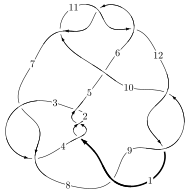
\includegraphics[width=112pt]{../../../GIT/diagram.site/Diagrams/png/1628_12a_0827.png}\\
\ \ \ A knot diagram\footnotemark}&
\allowdisplaybreaks
\textbf{Linearized knot diagam} \\
\cline{2-2}
 &
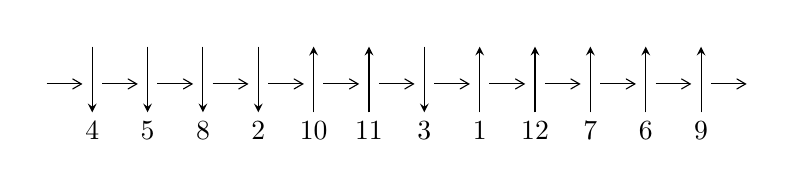
\begin{tikzpicture}[x=20pt, y=17pt]
	% nodes
	\node (C0) at (0, 0) {};
	\node (C1) at (1, 0) {};
	\node (C1U) at (1, +1) {};
	\node (C1D) at (1, -1) {4};

	\node (C2) at (2, 0) {};
	\node (C2U) at (2, +1) {};
	\node (C2D) at (2, -1) {5};

	\node (C3) at (3, 0) {};
	\node (C3U) at (3, +1) {};
	\node (C3D) at (3, -1) {8};

	\node (C4) at (4, 0) {};
	\node (C4U) at (4, +1) {};
	\node (C4D) at (4, -1) {2};

	\node (C5) at (5, 0) {};
	\node (C5U) at (5, +1) {};
	\node (C5D) at (5, -1) {10};

	\node (C6) at (6, 0) {};
	\node (C6U) at (6, +1) {};
	\node (C6D) at (6, -1) {11};

	\node (C7) at (7, 0) {};
	\node (C7U) at (7, +1) {};
	\node (C7D) at (7, -1) {3};

	\node (C8) at (8, 0) {};
	\node (C8U) at (8, +1) {};
	\node (C8D) at (8, -1) {1};

	\node (C9) at (9, 0) {};
	\node (C9U) at (9, +1) {};
	\node (C9D) at (9, -1) {12};

	\node (C10) at (10, 0) {};
	\node (C10U) at (10, +1) {};
	\node (C10D) at (10, -1) {7};

	\node (C11) at (11, 0) {};
	\node (C11U) at (11, +1) {};
	\node (C11D) at (11, -1) {6};

	\node (C12) at (12, 0) {};
	\node (C12U) at (12, +1) {};
	\node (C12D) at (12, -1) {9};
	\node (C13) at (13, 0) {};

	% arrows
	\draw[->,>={angle 60}]
	(C0) edge (C1) (C1) edge (C2) (C2) edge (C3) (C3) edge (C4) (C4) edge (C5) (C5) edge (C6) (C6) edge (C7) (C7) edge (C8) (C8) edge (C9) (C9) edge (C10) (C10) edge (C11) (C11) edge (C12) (C12) edge (C13) ;	\draw[->,>=stealth]
	(C1U) edge (C1D) (C2U) edge (C2D) (C3U) edge (C3D) (C4U) edge (C4D) (C5D) edge (C5U) (C6D) edge (C6U) (C7U) edge (C7D) (C8D) edge (C8U) (C9D) edge (C9U) (C10D) edge (C10U) (C11D) edge (C11U) (C12D) edge (C12U) ;
	\end{tikzpicture} \\
\hhline{~~} \\& 
\textbf{Solving Sequence} \\ \cline{2-2} 
 &
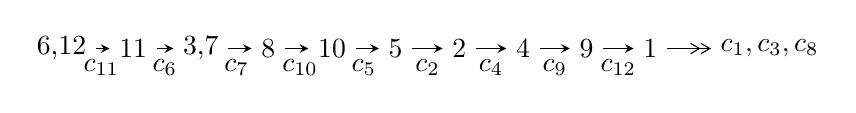
\begin{tikzpicture}[x=23pt, y=7pt]
	% node
	\node (A0) at (-1/8, 0) {6,12};
	\node (A1) at (1, 0) {11};
	\node (A2) at (33/16, 0) {3,7};
	\node (A3) at (25/8, 0) {8};
	\node (A4) at (33/8, 0) {10};
	\node (A5) at (41/8, 0) {5};
	\node (A6) at (49/8, 0) {2};
	\node (A7) at (57/8, 0) {4};
	\node (A8) at (65/8, 0) {9};
	\node (A9) at (73/8, 0) {1};
	\node (C1) at (1/2, -1) {$c_{11}$};
	\node (C2) at (3/2, -1) {$c_{6}$};
	\node (C3) at (21/8, -1) {$c_{7}$};
	\node (C4) at (29/8, -1) {$c_{10}$};
	\node (C5) at (37/8, -1) {$c_{5}$};
	\node (C6) at (45/8, -1) {$c_{2}$};
	\node (C7) at (53/8, -1) {$c_{4}$};
	\node (C8) at (61/8, -1) {$c_{9}$};
	\node (C9) at (69/8, -1) {$c_{12}$};
	\node (A10) at (11, 0) {$c_{1},c_{3},c_{8}$};

	% edge
	\draw[->,>=stealth]	
	(A0) edge (A1) (A1) edge (A2) (A2) edge (A3) (A3) edge (A4) (A4) edge (A5) (A5) edge (A6) (A6) edge (A7) (A7) edge (A8) (A8) edge (A9) ;
	\draw[->>,>={angle 60}]	
	(A9) edge (A10);
\end{tikzpicture} \\ 

\end{tabular} \\

\footnotetext{
The image of knot diagram is generated by the software ``\textbf{Draw programme}" developed by Andrew Bartholomew(\url{http://www.layer8.co.uk/maths/draw/index.htm\#Running-draw}), where we modified some parts for our purpose(\url{https://github.com/CATsTAILs/LinksPainter}).
}\phantom \\ \newline 
\centering \textbf{Ideals for irreducible components\footnotemark of $X_{\text{par}}$} 
 
\begin{align*}
I^u_{1}&=\langle 
u^{53}+u^{52}+\cdots+b-3 u,\;- u^{53}+u^{52}+\cdots+a+1,\;u^{56}-2 u^{55}+\cdots- u-1\rangle \\
I^u_{2}&=\langle 
- u^2+b-1,\;a-1,\;u^3+2 u-1\rangle \\
I^u_{3}&=\langle 
u^3+u^2+b+u+1,\;a+u+1,\;u^4+u^3+2 u^2+2 u+1\rangle \\
\\
\end{align*}
\raggedright * 3 irreducible components of $\dim_{\mathbb{C}}=0$, with total 63 representations.\\
\footnotetext{All coefficients of polynomials are rational numbers. But the coefficients are sometimes approximated in decimal forms when there is not enough margin.}
\newpage
\renewcommand{\arraystretch}{1}
\centering \section*{I. $I^u_{1}= \langle u^{53}+u^{52}+\cdots+b-3 u,\;- u^{53}+u^{52}+\cdots+a+1,\;u^{56}-2 u^{55}+\cdots- u-1 \rangle$}
\flushleft \textbf{(i) Arc colorings}\\
\begin{tabular}{m{7pt} m{180pt} m{7pt} m{180pt} }
\flushright $a_{6}=$&$\begin{pmatrix}0\\u\end{pmatrix}$ \\
\flushright $a_{12}=$&$\begin{pmatrix}1\\0\end{pmatrix}$ \\
\flushright $a_{11}=$&$\begin{pmatrix}1\\u^2\end{pmatrix}$ \\
\flushright $a_{3}=$&$\begin{pmatrix}u^{53}- u^{52}+\cdots+5 u-1\\- u^{53}- u^{52}+\cdots-2 u^2+3 u\end{pmatrix}$ \\
\flushright $a_{7}=$&$\begin{pmatrix}u\\u^3+u\end{pmatrix}$ \\
\flushright $a_{8}=$&$\begin{pmatrix}- u^{12}-5 u^{10}-7 u^8+2 u^4-3 u^2+1\\u^{12}+6 u^{10}+12 u^8+8 u^6+u^4+2 u^2\end{pmatrix}$ \\
\flushright $a_{10}=$&$\begin{pmatrix}u^2+1\\u^4+2 u^2\end{pmatrix}$ \\
\flushright $a_{5}=$&$\begin{pmatrix}- u^5-2 u^3- u\\- u^7-3 u^5-2 u^3+u\end{pmatrix}$ \\
\flushright $a_{2}=$&$\begin{pmatrix}- u^{50}+u^{49}+\cdots+3 u-2\\- u^{52}+u^{51}+\cdots-3 u^2+2 u\end{pmatrix}$ \\
\flushright $a_{4}=$&$\begin{pmatrix}- u^{53}+u^{52}+\cdots+u-2\\u^{53}- u^{52}+\cdots-5 u^2+2 u\end{pmatrix}$ \\
\flushright $a_{9}=$&$\begin{pmatrix}- u^4- u^2+1\\u^4+2 u^2\end{pmatrix}$ \\
\flushright $a_{1}=$&$\begin{pmatrix}u^8+3 u^6+u^4-2 u^2+1\\- u^8-4 u^6-4 u^4\end{pmatrix}$\\&\end{tabular}
\flushleft \textbf{(ii) Obstruction class $= -1$}\\~\\
\flushleft \textbf{(iii) Cusp Shapes $= 4 u^{55}-8 u^{54}+\cdots+41 u+1$}\\~\\
\newpage\renewcommand{\arraystretch}{1}
\flushleft \textbf{(iv) u-Polynomials at the component}\newline \\
\begin{tabular}{m{50pt}|m{274pt}}
Crossings & \hspace{64pt}u-Polynomials at each crossing \\
\hline $$\begin{aligned}c_{1},c_{2},c_{4}\end{aligned}$$&$\begin{aligned}
&u^{56}-8 u^{55}+\cdots+4 u-1
\end{aligned}$\\
\hline $$\begin{aligned}c_{3},c_{7}\end{aligned}$$&$\begin{aligned}
&u^{56}- u^{55}+\cdots+64 u+128
\end{aligned}$\\
\hline $$\begin{aligned}c_{5}\end{aligned}$$&$\begin{aligned}
&u^{56}+2 u^{55}+\cdots-6840 u-1480
\end{aligned}$\\
\hline $$\begin{aligned}c_{6},c_{10},c_{11}\end{aligned}$$&$\begin{aligned}
&u^{56}-2 u^{55}+\cdots- u-1
\end{aligned}$\\
\hline $$\begin{aligned}c_{8},c_{9},c_{12}\end{aligned}$$&$\begin{aligned}
&u^{56}+6 u^{55}+\cdots+15 u+19
\end{aligned}$\\
\hline
\end{tabular}\\~\\
\newpage\renewcommand{\arraystretch}{1}
\flushleft \textbf{(v) Riley Polynomials at the component}\newline \\
\begin{tabular}{m{50pt}|m{274pt}}
Crossings & \hspace{64pt}Riley Polynomials at each crossing \\
\hline $$\begin{aligned}c_{1},c_{2},c_{4}\end{aligned}$$&$\begin{aligned}
&y^{56}-60 y^{55}+\cdots+20 y+1
\end{aligned}$\\
\hline $$\begin{aligned}c_{3},c_{7}\end{aligned}$$&$\begin{aligned}
&y^{56}-45 y^{55}+\cdots-77824 y+16384
\end{aligned}$\\
\hline $$\begin{aligned}c_{5}\end{aligned}$$&$\begin{aligned}
&y^{56}+30 y^{55}+\cdots+5106160 y+2190400
\end{aligned}$\\
\hline $$\begin{aligned}c_{6},c_{10},c_{11}\end{aligned}$$&$\begin{aligned}
&y^{56}+54 y^{55}+\cdots-21 y+1
\end{aligned}$\\
\hline $$\begin{aligned}c_{8},c_{9},c_{12}\end{aligned}$$&$\begin{aligned}
&y^{56}+66 y^{55}+\cdots-9725 y+361
\end{aligned}$\\
\hline
\end{tabular}\\~\\
\newpage\flushleft \textbf{(vi) Complex Volumes and Cusp Shapes}
$$\begin{array}{c|c|c}  
\text{Solutions to }I^u_{1}& \I (\text{vol} + \sqrt{-1}CS) & \text{Cusp shape}\\
 \hline 
\begin{aligned}
u &= \phantom{-}0.660832 + 0.532382 I \\
a &= -2.01116 - 0.10615 I \\
b &= -0.35051 - 2.14768 I\end{aligned}
 & -15.9022 - 5.0365 I & -5.83411 + 0.48302 I \\ \hline\begin{aligned}
u &= \phantom{-}0.660832 - 0.532382 I \\
a &= -2.01116 + 0.10615 I \\
b &= -0.35051 + 2.14768 I\end{aligned}
 & -15.9022 + 5.0365 I & -5.83411 - 0.48302 I \\ \hline\begin{aligned}
u &= \phantom{-}0.708316 + 0.463836 I \\
a &= \phantom{-}1.259210 + 0.179633 I \\
b &= \phantom{-}0.37444 + 2.69166 I\end{aligned}
 & -15.6591 + 9.6036 I & -5.25563 - 6.20278 I \\ \hline\begin{aligned}
u &= \phantom{-}0.708316 - 0.463836 I \\
a &= \phantom{-}1.259210 - 0.179633 I \\
b &= \phantom{-}0.37444 - 2.69166 I\end{aligned}
 & -15.6591 - 9.6036 I & -5.25563 + 6.20278 I \\ \hline\begin{aligned}
u &= -0.676559 + 0.489617 I \\
a &= -0.386353 + 0.785496 I \\
b &= \phantom{-}1.073820 - 0.154726 I\end{aligned}
 & -10.73890 - 2.24941 I & -4.62574 + 2.95001 I \\ \hline\begin{aligned}
u &= -0.676559 - 0.489617 I \\
a &= -0.386353 - 0.785496 I \\
b &= \phantom{-}1.073820 + 0.154726 I\end{aligned}
 & -10.73890 + 2.24941 I & -4.62574 - 2.95001 I \\ \hline\begin{aligned}
u &= \phantom{-}0.682129 + 0.475711 I \\
a &= -1.55512 - 0.39032 I \\
b &= -0.49146 - 2.66606 I\end{aligned}
 & -8.46348 + 5.18228 I & -3.67010 - 5.70178 I \\ \hline\begin{aligned}
u &= \phantom{-}0.682129 - 0.475711 I \\
a &= -1.55512 + 0.39032 I \\
b &= -0.49146 + 2.66606 I\end{aligned}
 & -8.46348 - 5.18228 I & -3.67010 + 5.70178 I \\ \hline\begin{aligned}
u &= \phantom{-}0.664199 + 0.499108 I \\
a &= \phantom{-}1.88326 + 0.30058 I \\
b &= \phantom{-}0.59126 + 2.40754 I\end{aligned}
 & -8.55005 - 0.70692 I & -4.00146 - 0.24980 I \\ \hline\begin{aligned}
u &= \phantom{-}0.664199 - 0.499108 I \\
a &= \phantom{-}1.88326 - 0.30058 I \\
b &= \phantom{-}0.59126 - 2.40754 I\end{aligned}
 & -8.55005 + 0.70692 I & -4.00146 + 0.24980 I\\
 \hline 
 \end{array}$$\newpage$$\begin{array}{c|c|c}  
\text{Solutions to }I^u_{1}& \I (\text{vol} + \sqrt{-1}CS) & \text{Cusp shape}\\
 \hline 
\begin{aligned}
u &= \phantom{-}0.185528 + 1.194610 I \\
a &= \phantom{-}1.15155 + 1.06757 I \\
b &= -0.869359 - 0.937264 I\end{aligned}
 & -7.53088 + 3.11306 I & \phantom{-0.000000 } 0 \\ \hline\begin{aligned}
u &= \phantom{-}0.185528 - 1.194610 I \\
a &= \phantom{-}1.15155 - 1.06757 I \\
b &= -0.869359 + 0.937264 I\end{aligned}
 & -7.53088 - 3.11306 I & \phantom{-0.000000 } 0 \\ \hline\begin{aligned}
u &= -0.634915 + 0.454764 I \\
a &= \phantom{-}0.148473 - 0.390436 I \\
b &= -0.506435 + 0.067605 I\end{aligned}
 & -3.97803 - 2.08824 I & \phantom{-}3.15083 + 3.45018 I \\ \hline\begin{aligned}
u &= -0.634915 - 0.454764 I \\
a &= \phantom{-}0.148473 + 0.390436 I \\
b &= -0.506435 - 0.067605 I\end{aligned}
 & -3.97803 + 2.08824 I & \phantom{-}3.15083 - 3.45018 I \\ \hline\begin{aligned}
u &= \phantom{-}0.066056 + 1.253010 I \\
a &= -1.231350 - 0.008674 I \\
b &= \phantom{-}1.006180 + 0.304650 I\end{aligned}
 & -2.42783 + 1.72439 I & \phantom{-0.000000 } 0 \\ \hline\begin{aligned}
u &= \phantom{-}0.066056 - 1.253010 I \\
a &= -1.231350 + 0.008674 I \\
b &= \phantom{-}1.006180 - 0.304650 I\end{aligned}
 & -2.42783 - 1.72439 I & \phantom{-0.000000 } 0 \\ \hline\begin{aligned}
u &= -0.658902 + 0.263840 I \\
a &= -0.849914 + 0.073788 I \\
b &= \phantom{-}0.44012 + 1.55766 I\end{aligned}
 & -6.76817 - 5.79426 I & -2.57901 + 6.54647 I \\ \hline\begin{aligned}
u &= -0.658902 - 0.263840 I \\
a &= -0.849914 - 0.073788 I \\
b &= \phantom{-}0.44012 - 1.55766 I\end{aligned}
 & -6.76817 + 5.79426 I & -2.57901 - 6.54647 I \\ \hline\begin{aligned}
u &= -0.355604 + 0.604584 I \\
a &= \phantom{-}1.27737 + 1.18185 I \\
b &= \phantom{-}0.176477 - 1.192730 I\end{aligned}
 & -8.09448 + 2.23237 I & -6.24032 - 0.17719 I \\ \hline\begin{aligned}
u &= -0.355604 - 0.604584 I \\
a &= \phantom{-}1.27737 - 1.18185 I \\
b &= \phantom{-}0.176477 + 1.192730 I\end{aligned}
 & -8.09448 - 2.23237 I & -6.24032 + 0.17719 I\\
 \hline 
 \end{array}$$\newpage$$\begin{array}{c|c|c}  
\text{Solutions to }I^u_{1}& \I (\text{vol} + \sqrt{-1}CS) & \text{Cusp shape}\\
 \hline 
\begin{aligned}
u &= -0.032180 + 1.315600 I \\
a &= \phantom{-}1.65049 - 1.49020 I \\
b &= -1.72250 + 0.53274 I\end{aligned}
 & -5.16815 - 0.97608 I & \phantom{-0.000000 } 0 \\ \hline\begin{aligned}
u &= -0.032180 - 1.315600 I \\
a &= \phantom{-}1.65049 + 1.49020 I \\
b &= -1.72250 - 0.53274 I\end{aligned}
 & -5.16815 + 0.97608 I & \phantom{-0.000000 } 0 \\ \hline\begin{aligned}
u &= \phantom{-}0.140776 + 1.329860 I \\
a &= \phantom{-}0.112471 - 0.618255 I \\
b &= -0.251370 + 0.625724 I\end{aligned}
 & -3.44679 + 2.43795 I & \phantom{-0.000000 } 0 \\ \hline\begin{aligned}
u &= \phantom{-}0.140776 - 1.329860 I \\
a &= \phantom{-}0.112471 + 0.618255 I \\
b &= -0.251370 - 0.625724 I\end{aligned}
 & -3.44679 - 2.43795 I & \phantom{-0.000000 } 0 \\ \hline\begin{aligned}
u &= \phantom{-}0.650158\phantom{ +0.000000I} \\
a &= \phantom{-}0.687504\phantom{ +0.000000I} \\
b &= -0.940476\phantom{ +0.000000I}\end{aligned}
 & -3.94742\phantom{ +0.000000I} & \phantom{-}0.365180\phantom{ +0.000000I} \\ \hline\begin{aligned}
u &= -0.550030 + 0.257011 I \\
a &= \phantom{-}1.005750 - 0.053759 I \\
b &= \phantom{-}0.08417 - 1.41533 I\end{aligned}
 & -0.60546 - 3.13990 I & \phantom{-}0.90903 + 8.93719 I \\ \hline\begin{aligned}
u &= -0.550030 - 0.257011 I \\
a &= \phantom{-}1.005750 + 0.053759 I \\
b &= \phantom{-}0.08417 + 1.41533 I\end{aligned}
 & -0.60546 + 3.13990 I & \phantom{-}0.90903 - 8.93719 I \\ \hline\begin{aligned}
u &= -0.194330 + 1.384330 I \\
a &= \phantom{-}1.52389 + 1.96311 I \\
b &= -0.42665 - 1.78739 I\end{aligned}
 & -5.81737 - 5.85679 I & \phantom{-0.000000 } 0 \\ \hline\begin{aligned}
u &= -0.194330 - 1.384330 I \\
a &= \phantom{-}1.52389 - 1.96311 I \\
b &= -0.42665 + 1.78739 I\end{aligned}
 & -5.81737 + 5.85679 I & \phantom{-0.000000 } 0 \\ \hline\begin{aligned}
u &= -0.244927 + 1.385240 I \\
a &= -2.01842 - 1.29418 I \\
b &= \phantom{-}0.99243 + 1.48272 I\end{aligned}
 & -11.9991 - 9.0718 I & \phantom{-0.000000 } 0\\
 \hline 
 \end{array}$$\newpage$$\begin{array}{c|c|c}  
\text{Solutions to }I^u_{1}& \I (\text{vol} + \sqrt{-1}CS) & \text{Cusp shape}\\
 \hline 
\begin{aligned}
u &= -0.244927 - 1.385240 I \\
a &= -2.01842 + 1.29418 I \\
b &= \phantom{-}0.99243 - 1.48272 I\end{aligned}
 & -11.9991 + 9.0718 I & \phantom{-0.000000 } 0 \\ \hline\begin{aligned}
u &= -0.135589 + 1.401420 I \\
a &= -0.55425 - 2.40672 I \\
b &= -0.40949 + 1.76759 I\end{aligned}
 & -6.82917 - 1.43395 I & \phantom{-0.000000 } 0 \\ \hline\begin{aligned}
u &= -0.135589 - 1.401420 I \\
a &= -0.55425 + 2.40672 I \\
b &= -0.40949 - 1.76759 I\end{aligned}
 & -6.82917 + 1.43395 I & \phantom{-0.000000 } 0 \\ \hline\begin{aligned}
u &= \phantom{-}0.169908 + 1.402300 I \\
a &= -0.588451 + 0.710634 I \\
b &= \phantom{-}0.950712 - 1.025380 I\end{aligned}
 & -8.25453 + 3.79866 I & \phantom{-0.000000 } 0 \\ \hline\begin{aligned}
u &= \phantom{-}0.169908 - 1.402300 I \\
a &= -0.588451 - 0.710634 I \\
b &= \phantom{-}0.950712 + 1.025380 I\end{aligned}
 & -8.25453 - 3.79866 I & \phantom{-0.000000 } 0 \\ \hline\begin{aligned}
u &= \phantom{-}0.477090 + 0.308383 I \\
a &= \phantom{-}1.096420 + 0.178210 I \\
b &= \phantom{-}0.155533 - 0.573459 I\end{aligned}
 & -2.81186 + 1.40524 I & -1.32654 - 4.47405 I \\ \hline\begin{aligned}
u &= \phantom{-}0.477090 - 0.308383 I \\
a &= \phantom{-}1.096420 - 0.178210 I \\
b &= \phantom{-}0.155533 + 0.573459 I\end{aligned}
 & -2.81186 - 1.40524 I & -1.32654 + 4.47405 I \\ \hline\begin{aligned}
u &= -0.09346 + 1.46417 I \\
a &= \phantom{-}0.20672 + 1.99781 I \\
b &= \phantom{-}0.533413 - 1.285270 I\end{aligned}
 & -14.6540 + 0.7423 I & \phantom{-0.000000 } 0 \\ \hline\begin{aligned}
u &= -0.09346 - 1.46417 I \\
a &= \phantom{-}0.20672 - 1.99781 I \\
b &= \phantom{-}0.533413 + 1.285270 I\end{aligned}
 & -14.6540 - 0.7423 I & \phantom{-0.000000 } 0 \\ \hline\begin{aligned}
u &= -0.22823 + 1.47473 I \\
a &= \phantom{-}0.447474 - 0.510871 I \\
b &= -0.437565 + 0.216954 I\end{aligned}
 & -10.20770 - 5.24287 I & \phantom{-0.000000 } 0\\
 \hline 
 \end{array}$$\newpage$$\begin{array}{c|c|c}  
\text{Solutions to }I^u_{1}& \I (\text{vol} + \sqrt{-1}CS) & \text{Cusp shape}\\
 \hline 
\begin{aligned}
u &= -0.22823 - 1.47473 I \\
a &= \phantom{-}0.447474 + 0.510871 I \\
b &= -0.437565 - 0.216954 I\end{aligned}
 & -10.20770 + 5.24287 I & \phantom{-0.000000 } 0 \\ \hline\begin{aligned}
u &= \phantom{-}0.482677 + 0.077215 I \\
a &= -0.481205 - 0.248126 I \\
b &= \phantom{-}0.246960 + 0.272043 I\end{aligned}
 & \phantom{-}0.970388 + 0.223799 I & \phantom{-}9.84475 - 1.11489 I \\ \hline\begin{aligned}
u &= \phantom{-}0.482677 - 0.077215 I \\
a &= -0.481205 + 0.248126 I \\
b &= \phantom{-}0.246960 - 0.272043 I\end{aligned}
 & \phantom{-}0.970388 - 0.223799 I & \phantom{-}9.84475 + 1.11489 I \\ \hline\begin{aligned}
u &= \phantom{-}0.24142 + 1.49209 I \\
a &= -0.96174 + 3.18550 I \\
b &= -1.14574 - 3.47762 I\end{aligned}
 & -14.8427 + 8.5522 I & \phantom{-0.000000 } 0 \\ \hline\begin{aligned}
u &= \phantom{-}0.24142 - 1.49209 I \\
a &= -0.96174 - 3.18550 I \\
b &= -1.14574 + 3.47762 I\end{aligned}
 & -14.8427 - 8.5522 I & \phantom{-0.000000 } 0 \\ \hline\begin{aligned}
u &= \phantom{-}0.25422 + 1.49240 I \\
a &= \phantom{-}1.26227 - 3.10390 I \\
b &= \phantom{-}0.62907 + 3.47790 I\end{aligned}
 & \phantom{-}17.4812 + 13.1175 I & \phantom{-0.000000 } 0 \\ \hline\begin{aligned}
u &= \phantom{-}0.25422 - 1.49240 I \\
a &= \phantom{-}1.26227 + 3.10390 I \\
b &= \phantom{-}0.62907 - 3.47790 I\end{aligned}
 & \phantom{-}17.4812 - 13.1175 I & \phantom{-0.000000 } 0 \\ \hline\begin{aligned}
u &= \phantom{-}0.22938 + 1.49684 I \\
a &= \phantom{-}0.54325 - 2.87749 I \\
b &= \phantom{-}1.58029 + 2.89554 I\end{aligned}
 & -15.0303 + 2.5470 I & \phantom{-0.000000 } 0 \\ \hline\begin{aligned}
u &= \phantom{-}0.22938 - 1.49684 I \\
a &= \phantom{-}0.54325 + 2.87749 I \\
b &= \phantom{-}1.58029 - 2.89554 I\end{aligned}
 & -15.0303 - 2.5470 I & \phantom{-0.000000 } 0 \\ \hline\begin{aligned}
u &= -0.23625 + 1.49620 I \\
a &= -0.956299 + 1.041640 I \\
b &= \phantom{-}0.911847 - 0.439648 I\end{aligned}
 & -17.1840 - 5.5773 I & \phantom{-0.000000 } 0\\
 \hline 
 \end{array}$$\newpage$$\begin{array}{c|c|c}  
\text{Solutions to }I^u_{1}& \I (\text{vol} + \sqrt{-1}CS) & \text{Cusp shape}\\
 \hline 
\begin{aligned}
u &= -0.23625 - 1.49620 I \\
a &= -0.956299 - 1.041640 I \\
b &= \phantom{-}0.911847 + 0.439648 I\end{aligned}
 & -17.1840 + 5.5773 I & \phantom{-0.000000 } 0 \\ \hline\begin{aligned}
u &= -0.328861 + 0.345682 I \\
a &= -1.49250 - 0.54755 I \\
b &= -0.337925 + 0.940882 I\end{aligned}
 & -1.35678 + 0.40897 I & -4.58141 + 0.13803 I \\ \hline\begin{aligned}
u &= -0.328861 - 0.345682 I \\
a &= -1.49250 + 0.54755 I \\
b &= -0.337925 - 0.940882 I\end{aligned}
 & -1.35678 - 0.40897 I & -4.58141 - 0.13803 I \\ \hline\begin{aligned}
u &= \phantom{-}0.21901 + 1.50844 I \\
a &= -0.60237 + 2.27231 I \\
b &= -1.30465 - 2.19638 I\end{aligned}
 & \phantom{-}16.9245 - 1.8446 I & \phantom{-0.000000 } 0 \\ \hline\begin{aligned}
u &= \phantom{-}0.21901 - 1.50844 I \\
a &= -0.60237 - 2.27231 I \\
b &= -1.30465 + 2.19638 I\end{aligned}
 & \phantom{-}16.9245 + 1.8446 I & \phantom{-0.000000 } 0 \\ \hline\begin{aligned}
u &= -0.273566\phantom{ +0.000000I} \\
a &= -2.44641\phantom{ +0.000000I} \\
b &= -1.04562\phantom{ +0.000000I}\end{aligned}
 & -1.24400\phantom{ +0.000000I} & -12.1870\phantom{ +0.000000I}\\
 \hline 
 \end{array}$$\newpage\newpage\renewcommand{\arraystretch}{1}
\centering \section*{II. $I^u_{2}= \langle - u^2+b-1,\;a-1,\;u^3+2 u-1 \rangle$}
\flushleft \textbf{(i) Arc colorings}\\
\begin{tabular}{m{7pt} m{180pt} m{7pt} m{180pt} }
\flushright $a_{6}=$&$\begin{pmatrix}0\\u\end{pmatrix}$ \\
\flushright $a_{12}=$&$\begin{pmatrix}1\\0\end{pmatrix}$ \\
\flushright $a_{11}=$&$\begin{pmatrix}1\\u^2\end{pmatrix}$ \\
\flushright $a_{3}=$&$\begin{pmatrix}1\\u^2+1\end{pmatrix}$ \\
\flushright $a_{7}=$&$\begin{pmatrix}u\\- u+1\end{pmatrix}$ \\
\flushright $a_{8}=$&$\begin{pmatrix}u\\- u+1\end{pmatrix}$ \\
\flushright $a_{10}=$&$\begin{pmatrix}u^2+1\\u\end{pmatrix}$ \\
\flushright $a_{5}=$&$\begin{pmatrix}- u^2- u\\u^2\end{pmatrix}$ \\
\flushright $a_{2}=$&$\begin{pmatrix}u^2+u+1\\1\end{pmatrix}$ \\
\flushright $a_{4}=$&$\begin{pmatrix}1\\u^2+1\end{pmatrix}$ \\
\flushright $a_{9}=$&$\begin{pmatrix}u^2- u+1\\u\end{pmatrix}$ \\
\flushright $a_{1}=$&$\begin{pmatrix}u^2+u\\- u^2\end{pmatrix}$\\&\end{tabular}
\flushleft \textbf{(ii) Obstruction class $= 1$}\\~\\
\flushleft \textbf{(iii) Cusp Shapes $= 7 u^2+5 u+6$}\\~\\
\newpage\renewcommand{\arraystretch}{1}
\flushleft \textbf{(iv) u-Polynomials at the component}\newline \\
\begin{tabular}{m{50pt}|m{274pt}}
Crossings & \hspace{64pt}u-Polynomials at each crossing \\
\hline $$\begin{aligned}c_{1},c_{2}\end{aligned}$$&$\begin{aligned}
&(u-1)^3
\end{aligned}$\\
\hline $$\begin{aligned}c_{3},c_{7}\end{aligned}$$&$\begin{aligned}
&u^3
\end{aligned}$\\
\hline $$\begin{aligned}c_{4}\end{aligned}$$&$\begin{aligned}
&(u+1)^3
\end{aligned}$\\
\hline $$\begin{aligned}c_{5}\end{aligned}$$&$\begin{aligned}
&u^3+3 u^2+5 u+2
\end{aligned}$\\
\hline $$\begin{aligned}c_{6},c_{8},c_{9}\end{aligned}$$&$\begin{aligned}
&u^3+2 u+1
\end{aligned}$\\
\hline $$\begin{aligned}c_{10},c_{11},c_{12}\end{aligned}$$&$\begin{aligned}
&u^3+2 u-1
\end{aligned}$\\
\hline
\end{tabular}\\~\\
\newpage\renewcommand{\arraystretch}{1}
\flushleft \textbf{(v) Riley Polynomials at the component}\newline \\
\begin{tabular}{m{50pt}|m{274pt}}
Crossings & \hspace{64pt}Riley Polynomials at each crossing \\
\hline $$\begin{aligned}c_{1},c_{2},c_{4}\end{aligned}$$&$\begin{aligned}
&(y-1)^3
\end{aligned}$\\
\hline $$\begin{aligned}c_{3},c_{7}\end{aligned}$$&$\begin{aligned}
&y^3
\end{aligned}$\\
\hline $$\begin{aligned}c_{5}\end{aligned}$$&$\begin{aligned}
&y^3+y^2+13 y-4
\end{aligned}$\\
\hline $$\begin{aligned}c_{6},c_{8},c_{9}\\c_{10},c_{11},c_{12}\end{aligned}$$&$\begin{aligned}
&y^3+4 y^2+4 y-1
\end{aligned}$\\
\hline
\end{tabular}\\~\\
\newpage\flushleft \textbf{(vi) Complex Volumes and Cusp Shapes}
$$\begin{array}{c|c|c}  
\text{Solutions to }I^u_{2}& \I (\text{vol} + \sqrt{-1}CS) & \text{Cusp shape}\\
 \hline 
\begin{aligned}
u &= -0.22670 + 1.46771 I \\
a &= \phantom{-}1.00000\phantom{ +0.000000I} \\
b &= -1.102790 - 0.665457 I\end{aligned}
 & -11.08570 - 5.13794 I & -9.85299 + 2.68036 I \\ \hline\begin{aligned}
u &= -0.22670 - 1.46771 I \\
a &= \phantom{-}1.00000\phantom{ +0.000000I} \\
b &= -1.102790 + 0.665457 I\end{aligned}
 & -11.08570 + 5.13794 I & -9.85299 - 2.68036 I \\ \hline\begin{aligned}
u &= \phantom{-}0.453398\phantom{ +0.000000I} \\
a &= \phantom{-}1.00000\phantom{ +0.000000I} \\
b &= \phantom{-}1.20557\phantom{ +0.000000I}\end{aligned}
 & -0.857735\phantom{ +0.000000I} & \phantom{-}9.70600\phantom{ +0.000000I}\\
 \hline 
 \end{array}$$\newpage\newpage\renewcommand{\arraystretch}{1}
\centering \section*{III. $I^u_{3}= \langle u^3+u^2+b+u+1,\;a+u+1,\;u^4+u^3+2 u^2+2 u+1 \rangle$}
\flushleft \textbf{(i) Arc colorings}\\
\begin{tabular}{m{7pt} m{180pt} m{7pt} m{180pt} }
\flushright $a_{6}=$&$\begin{pmatrix}0\\u\end{pmatrix}$ \\
\flushright $a_{12}=$&$\begin{pmatrix}1\\0\end{pmatrix}$ \\
\flushright $a_{11}=$&$\begin{pmatrix}1\\u^2\end{pmatrix}$ \\
\flushright $a_{3}=$&$\begin{pmatrix}- u-1\\- u^3- u^2- u-1\end{pmatrix}$ \\
\flushright $a_{7}=$&$\begin{pmatrix}u\\u^3+u\end{pmatrix}$ \\
\flushright $a_{8}=$&$\begin{pmatrix}u\\u^3+u\end{pmatrix}$ \\
\flushright $a_{10}=$&$\begin{pmatrix}u^2+1\\- u^3-2 u-1\end{pmatrix}$ \\
\flushright $a_{5}=$&$\begin{pmatrix}- u^3-2 u-1\\- u^3- u^2- u-2\end{pmatrix}$ \\
\flushright $a_{2}=$&$\begin{pmatrix}u^3+u\\1\end{pmatrix}$ \\
\flushright $a_{4}=$&$\begin{pmatrix}- u-1\\- u^3- u^2- u-1\end{pmatrix}$ \\
\flushright $a_{9}=$&$\begin{pmatrix}u^3+u^2+2 u+2\\- u^3-2 u-1\end{pmatrix}$ \\
\flushright $a_{1}=$&$\begin{pmatrix}u^3+2 u+1\\u^3+u^2+u+2\end{pmatrix}$\\&\end{tabular}
\flushleft \textbf{(ii) Obstruction class $= 1$}\\~\\
\flushleft \textbf{(iii) Cusp Shapes $= 3 u^3-2 u^2+2 u-5$}\\~\\
\newpage\renewcommand{\arraystretch}{1}
\flushleft \textbf{(iv) u-Polynomials at the component}\newline \\
\begin{tabular}{m{50pt}|m{274pt}}
Crossings & \hspace{64pt}u-Polynomials at each crossing \\
\hline $$\begin{aligned}c_{1},c_{2}\end{aligned}$$&$\begin{aligned}
&(u-1)^4
\end{aligned}$\\
\hline $$\begin{aligned}c_{3},c_{7}\end{aligned}$$&$\begin{aligned}
&u^4
\end{aligned}$\\
\hline $$\begin{aligned}c_{4}\end{aligned}$$&$\begin{aligned}
&(u+1)^4
\end{aligned}$\\
\hline $$\begin{aligned}c_{5}\end{aligned}$$&$\begin{aligned}
&(u^2- u+1)^2
\end{aligned}$\\
\hline $$\begin{aligned}c_{6},c_{8},c_{9}\end{aligned}$$&$\begin{aligned}
&u^4- u^3+2 u^2-2 u+1
\end{aligned}$\\
\hline $$\begin{aligned}c_{10},c_{11},c_{12}\end{aligned}$$&$\begin{aligned}
&u^4+u^3+2 u^2+2 u+1
\end{aligned}$\\
\hline
\end{tabular}\\~\\
\newpage\renewcommand{\arraystretch}{1}
\flushleft \textbf{(v) Riley Polynomials at the component}\newline \\
\begin{tabular}{m{50pt}|m{274pt}}
Crossings & \hspace{64pt}Riley Polynomials at each crossing \\
\hline $$\begin{aligned}c_{1},c_{2},c_{4}\end{aligned}$$&$\begin{aligned}
&(y-1)^4
\end{aligned}$\\
\hline $$\begin{aligned}c_{3},c_{7}\end{aligned}$$&$\begin{aligned}
&y^4
\end{aligned}$\\
\hline $$\begin{aligned}c_{5}\end{aligned}$$&$\begin{aligned}
&(y^2+y+1)^2
\end{aligned}$\\
\hline $$\begin{aligned}c_{6},c_{8},c_{9}\\c_{10},c_{11},c_{12}\end{aligned}$$&$\begin{aligned}
&y^4+3 y^3+2 y^2+1
\end{aligned}$\\
\hline
\end{tabular}\\~\\
\newpage\flushleft \textbf{(vi) Complex Volumes and Cusp Shapes}
$$\begin{array}{c|c|c}  
\text{Solutions to }I^u_{3}& \I (\text{vol} + \sqrt{-1}CS) & \text{Cusp shape}\\
 \hline 
\begin{aligned}
u &= -0.621744 + 0.440597 I \\
a &= -0.378256 - 0.440597 I \\
b &= -0.692440 - 0.318148 I\end{aligned}
 & -4.93480 - 2.02988 I & -6.26314 + 3.25323 I \\ \hline\begin{aligned}
u &= -0.621744 - 0.440597 I \\
a &= -0.378256 + 0.440597 I \\
b &= -0.692440 + 0.318148 I\end{aligned}
 & -4.93480 + 2.02988 I & -6.26314 - 3.25323 I \\ \hline\begin{aligned}
u &= \phantom{-}0.121744 + 1.306620 I \\
a &= -1.12174 - 1.30662 I \\
b &= \phantom{-}1.192440 + 0.547877 I\end{aligned}
 & -4.93480 + 2.02988 I & -3.23686 - 4.54099 I \\ \hline\begin{aligned}
u &= \phantom{-}0.121744 - 1.306620 I \\
a &= -1.12174 + 1.30662 I \\
b &= \phantom{-}1.192440 - 0.547877 I\end{aligned}
 & -4.93480 - 2.02988 I & -3.23686 + 4.54099 I\\
 \hline 
 \end{array}$$\newpage
\newpage\renewcommand{\arraystretch}{1}
\centering \section*{ IV. u-Polynomials}
\begin{tabular}{m{50pt}|m{274pt}}
Crossings & \hspace{64pt}u-Polynomials at each crossing \\
\hline $$\begin{aligned}c_{1},c_{2}\end{aligned}$$&$\begin{aligned}
&((u-1)^7)(u^{56}-8 u^{55}+\cdots+4 u-1)
\end{aligned}$\\
\hline $$\begin{aligned}c_{3},c_{7}\end{aligned}$$&$\begin{aligned}
&u^7(u^{56}- u^{55}+\cdots+64 u+128)
\end{aligned}$\\
\hline $$\begin{aligned}c_{4}\end{aligned}$$&$\begin{aligned}
&((u+1)^7)(u^{56}-8 u^{55}+\cdots+4 u-1)
\end{aligned}$\\
\hline $$\begin{aligned}c_{5}\end{aligned}$$&$\begin{aligned}
&((u^2- u+1)^2)(u^3+3 u^2+5 u+2)(u^{56}+2 u^{55}+\cdots-6840 u-1480)
\end{aligned}$\\
\hline $$\begin{aligned}c_{6}\end{aligned}$$&$\begin{aligned}
&(u^3+2 u+1)(u^4- u^3+2 u^2-2 u+1)(u^{56}-2 u^{55}+\cdots- u-1)
\end{aligned}$\\
\hline $$\begin{aligned}c_{8},c_{9}\end{aligned}$$&$\begin{aligned}
&(u^3+2 u+1)(u^4- u^3+2 u^2-2 u+1)(u^{56}+6 u^{55}+\cdots+15 u+19)
\end{aligned}$\\
\hline $$\begin{aligned}c_{10},c_{11}\end{aligned}$$&$\begin{aligned}
&(u^3+2 u-1)(u^4+u^3+2 u^2+2 u+1)(u^{56}-2 u^{55}+\cdots- u-1)
\end{aligned}$\\
\hline $$\begin{aligned}c_{12}\end{aligned}$$&$\begin{aligned}
&(u^3+2 u-1)(u^4+u^3+2 u^2+2 u+1)(u^{56}+6 u^{55}+\cdots+15 u+19)
\end{aligned}$\\
\hline
\end{tabular}\newpage\renewcommand{\arraystretch}{1}
\centering \section*{ V. Riley Polynomials}
\begin{tabular}{m{50pt}|m{274pt}}
Crossings & \hspace{64pt}Riley Polynomials at each crossing \\
\hline $$\begin{aligned}c_{1},c_{2},c_{4}\end{aligned}$$&$\begin{aligned}
&((y-1)^7)(y^{56}-60 y^{55}+\cdots+20 y+1)
\end{aligned}$\\
\hline $$\begin{aligned}c_{3},c_{7}\end{aligned}$$&$\begin{aligned}
&y^7(y^{56}-45 y^{55}+\cdots-77824 y+16384)
\end{aligned}$\\
\hline $$\begin{aligned}c_{5}\end{aligned}$$&$\begin{aligned}
&(y^2+y+1)^2(y^3+y^2+13 y-4)\\
&\cdot(y^{56}+30 y^{55}+\cdots+5106160 y+2190400)
\end{aligned}$\\
\hline $$\begin{aligned}c_{6},c_{10},c_{11}\end{aligned}$$&$\begin{aligned}
&(y^3+4 y^2+4 y-1)(y^4+3 y^3+2 y^2+1)(y^{56}+54 y^{55}+\cdots-21 y+1)
\end{aligned}$\\
\hline $$\begin{aligned}c_{8},c_{9},c_{12}\end{aligned}$$&$\begin{aligned}
&(y^3+4 y^2+4 y-1)(y^4+3 y^3+2 y^2+1)(y^{56}+66 y^{55}+\cdots-9725 y+361)
\end{aligned}$\\
\hline
\end{tabular}
\vskip 2pc
\end{document}